%!TEX root = ../../main.tex
\section{RS485 Converter}
RS485-bussen er valgt til at kommunikere på, se hvorfor i teknologiundersøgelsen. Systemet bygges op med hardware som kun understøtter RS232 kommunikation, det kræves derfor at der forekommer en konvertering til og fra RS485. Til dette formål er der udformet et simpelt kredsløb vha. MAX3082. Det logiske 0-5V RS232-signal konverteres til et differentielt signal, som kører ud på bussen, og vice versa.

\begin{figure}[H]
	\centering
	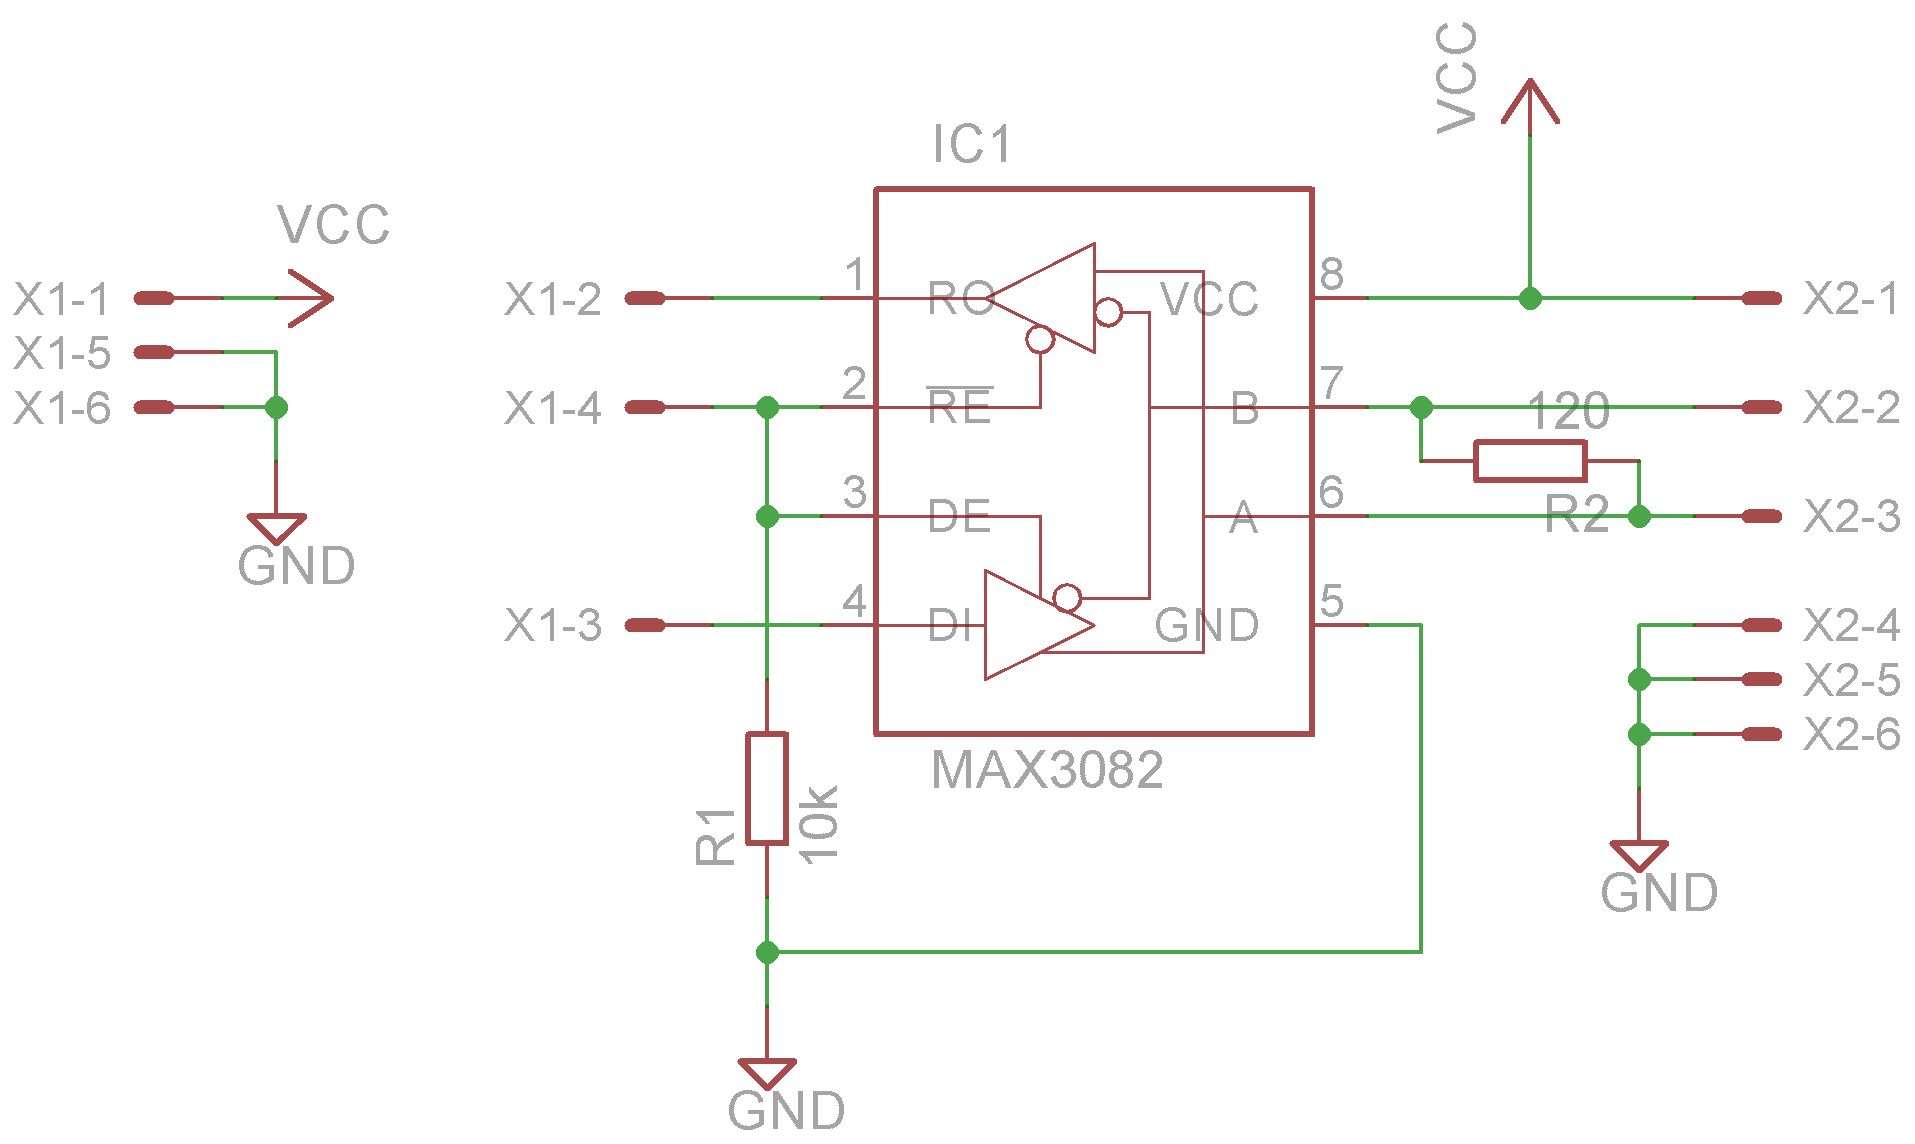
\includegraphics[scale=1]{../Hardware/RS485_Converter/Schematic}
	\caption{RS485 converter}
	\label{photo:RS485converter}
\end{figure}

\fxnote{Scopebilleder, forklaringer osv.}